\section{Results}

\subsection{Tagged sequential}

As described previously, the tagged sequential prefetcher was  implemented with
degree 5 and distance 4, as the performance  with this configuration proved to
be relatively good. The  resulting average speedup was 1.032. The ``ammp'' and
``twolf'' benchmarks gave  really bad results, with a speedup of respectively
0.759 and 0.983  (speedup below zero means the prefetcher actually slows down
the application). This is expected as those applications use large objects and
irregular cache alignment,  which makes it very challenging to predict future
memory accesses using spatial locality.

\todo[inline]{The results goes here.
\\
- Show that your scheme works\\
- Compare to other schemes that do the same thing. Hopefully you are better, but you need to compare anyway\\
Trick: “Oracle Scheme”\\
- Uses “perfect” information to create an upper bound on the
performance of a class of schemes\\
- Prefetching: Best case is that all L2 accesses are hits\\
Sensitivity analysis: \\
- Check the impact of model assumptions on your
scheme}

Our prefetcher was simulated with different combinations of degree and distance,
in the range of 0--6. The combination that got the best overall score on the
benchmark tests was with degree 5 and distance 4.

\begin{figure}[tbp]
\begin{center}
    % GNUPLOT: LaTeX picture with Postscript
\begingroup
  \makeatletter
  \providecommand\color[2][]{%
    \GenericError{(gnuplot) \space\space\space\@spaces}{%
      Package color not loaded in conjunction with
      terminal option `colourtext'%
    }{See the gnuplot documentation for explanation.%
    }{Either use 'blacktext' in gnuplot or load the package
      color.sty in LaTeX.}%
    \renewcommand\color[2][]{}%
  }%
  \providecommand\includegraphics[2][]{%
    \GenericError{(gnuplot) \space\space\space\@spaces}{%
      Package graphicx or graphics not loaded%
    }{See the gnuplot documentation for explanation.%
    }{The gnuplot epslatex terminal needs graphicx.sty or graphics.sty.}%
    \renewcommand\includegraphics[2][]{}%
  }%
  \providecommand\rotatebox[2]{#2}%
  \@ifundefined{ifGPcolor}{%
    \newif\ifGPcolor
    \GPcolorfalse
  }{}%
  \@ifundefined{ifGPblacktext}{%
    \newif\ifGPblacktext
    \GPblacktexttrue
  }{}%
  % define a \g@addto@macro without @ in the name:
  \let\gplgaddtomacro\g@addto@macro
  % define empty templates for all commands taking text:
  \gdef\gplbacktext{}%
  \gdef\gplfronttext{}%
  \makeatother
  \ifGPblacktext
    % no textcolor at all
    \def\colorrgb#1{}%
    \def\colorgray#1{}%
  \else
    % gray or color?
    \ifGPcolor
      \def\colorrgb#1{\color[rgb]{#1}}%
      \def\colorgray#1{\color[gray]{#1}}%
      \expandafter\def\csname LTw\endcsname{\color{white}}%
      \expandafter\def\csname LTb\endcsname{\color{black}}%
      \expandafter\def\csname LTa\endcsname{\color{black}}%
      \expandafter\def\csname LT0\endcsname{\color[rgb]{1,0,0}}%
      \expandafter\def\csname LT1\endcsname{\color[rgb]{0,1,0}}%
      \expandafter\def\csname LT2\endcsname{\color[rgb]{0,0,1}}%
      \expandafter\def\csname LT3\endcsname{\color[rgb]{1,0,1}}%
      \expandafter\def\csname LT4\endcsname{\color[rgb]{0,1,1}}%
      \expandafter\def\csname LT5\endcsname{\color[rgb]{1,1,0}}%
      \expandafter\def\csname LT6\endcsname{\color[rgb]{0,0,0}}%
      \expandafter\def\csname LT7\endcsname{\color[rgb]{1,0.3,0}}%
      \expandafter\def\csname LT8\endcsname{\color[rgb]{0.5,0.5,0.5}}%
    \else
      % gray
      \def\colorrgb#1{\color{black}}%
      \def\colorgray#1{\color[gray]{#1}}%
      \expandafter\def\csname LTw\endcsname{\color{white}}%
      \expandafter\def\csname LTb\endcsname{\color{black}}%
      \expandafter\def\csname LTa\endcsname{\color{black}}%
      \expandafter\def\csname LT0\endcsname{\color{black}}%
      \expandafter\def\csname LT1\endcsname{\color{black}}%
      \expandafter\def\csname LT2\endcsname{\color{black}}%
      \expandafter\def\csname LT3\endcsname{\color{black}}%
      \expandafter\def\csname LT4\endcsname{\color{black}}%
      \expandafter\def\csname LT5\endcsname{\color{black}}%
      \expandafter\def\csname LT6\endcsname{\color{black}}%
      \expandafter\def\csname LT7\endcsname{\color{black}}%
      \expandafter\def\csname LT8\endcsname{\color{black}}%
    \fi
  \fi
  \setlength{\unitlength}{0.0500bp}%
  \begin{picture}(5040.00,3528.00)%
    \gplgaddtomacro\gplbacktext{%
      \csname LTb\endcsname%
      \put(1078,704){\makebox(0,0)[r]{\strut{} 0.92}}%
      \put(1078,988){\makebox(0,0)[r]{\strut{} 0.94}}%
      \put(1078,1273){\makebox(0,0)[r]{\strut{} 0.96}}%
      \put(1078,1557){\makebox(0,0)[r]{\strut{} 0.98}}%
      \put(1078,1841){\makebox(0,0)[r]{\strut{} 1}}%
      \put(1078,2126){\makebox(0,0)[r]{\strut{} 1.02}}%
      \put(1078,2410){\makebox(0,0)[r]{\strut{} 1.04}}%
      \put(1078,2694){\makebox(0,0)[r]{\strut{} 1.06}}%
      \put(1078,2979){\makebox(0,0)[r]{\strut{} 1.08}}%
      \put(1078,3263){\makebox(0,0)[r]{\strut{} 1.1}}%
      \put(1591,484){\makebox(0,0){\strut{}2}}%
      \put(1973,484){\makebox(0,0){\strut{}4}}%
      \put(2354,484){\makebox(0,0){\strut{}6}}%
      \put(2736,484){\makebox(0,0){\strut{}8}}%
      \put(3117,484){\makebox(0,0){\strut{}10}}%
      \put(3499,484){\makebox(0,0){\strut{}12}}%
      \put(3880,484){\makebox(0,0){\strut{}14}}%
      \put(4262,484){\makebox(0,0){\strut{}16}}%
      \put(176,1983){\rotatebox{-270}{\makebox(0,0){\strut{}Speedup}}}%
      \put(2926,154){\makebox(0,0){\strut{}Distance}}%
    }%
    \gplgaddtomacro\gplfronttext{%
      \csname LTb\endcsname%
      \put(2197,3090){\makebox(0,0)[l]{\strut{}Degree = 1}}%
      \csname LTb\endcsname%
      \put(2197,2870){\makebox(0,0)[l]{\strut{}Degree = 2}}%
      \csname LTb\endcsname%
      \put(2197,2650){\makebox(0,0)[l]{\strut{}Degree = 3}}%
      \csname LTb\endcsname%
      \put(2197,2430){\makebox(0,0)[l]{\strut{}Degree = 4}}%
    }%
    \gplbacktext
    \put(0,0){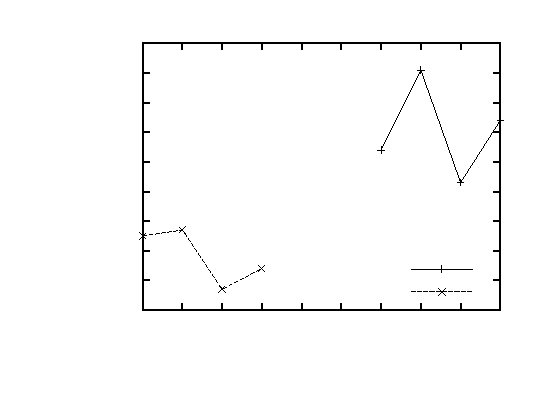
\includegraphics{tagged-sequential-plot}}%
    \gplfronttext
  \end{picture}%
\endgroup

    \caption{Speedup using the tagged sequential prefetcher}
    \label{graph:tagged-sequential}
\end{center}
\end{figure}

\begin{figure}[tbp]
\begin{center}
    % GNUPLOT: LaTeX picture with Postscript
\begingroup
  \makeatletter
  \providecommand\color[2][]{%
    \GenericError{(gnuplot) \space\space\space\@spaces}{%
      Package color not loaded in conjunction with
      terminal option `colourtext'%
    }{See the gnuplot documentation for explanation.%
    }{Either use 'blacktext' in gnuplot or load the package
      color.sty in LaTeX.}%
    \renewcommand\color[2][]{}%
  }%
  \providecommand\includegraphics[2][]{%
    \GenericError{(gnuplot) \space\space\space\@spaces}{%
      Package graphicx or graphics not loaded%
    }{See the gnuplot documentation for explanation.%
    }{The gnuplot epslatex terminal needs graphicx.sty or graphics.sty.}%
    \renewcommand\includegraphics[2][]{}%
  }%
  \providecommand\rotatebox[2]{#2}%
  \@ifundefined{ifGPcolor}{%
    \newif\ifGPcolor
    \GPcolorfalse
  }{}%
  \@ifundefined{ifGPblacktext}{%
    \newif\ifGPblacktext
    \GPblacktexttrue
  }{}%
  % define a \g@addto@macro without @ in the name:
  \let\gplgaddtomacro\g@addto@macro
  % define empty templates for all commands taking text:
  \gdef\gplbacktext{}%
  \gdef\gplfronttext{}%
  \makeatother
  \ifGPblacktext
    % no textcolor at all
    \def\colorrgb#1{}%
    \def\colorgray#1{}%
  \else
    % gray or color?
    \ifGPcolor
      \def\colorrgb#1{\color[rgb]{#1}}%
      \def\colorgray#1{\color[gray]{#1}}%
      \expandafter\def\csname LTw\endcsname{\color{white}}%
      \expandafter\def\csname LTb\endcsname{\color{black}}%
      \expandafter\def\csname LTa\endcsname{\color{black}}%
      \expandafter\def\csname LT0\endcsname{\color[rgb]{1,0,0}}%
      \expandafter\def\csname LT1\endcsname{\color[rgb]{0,1,0}}%
      \expandafter\def\csname LT2\endcsname{\color[rgb]{0,0,1}}%
      \expandafter\def\csname LT3\endcsname{\color[rgb]{1,0,1}}%
      \expandafter\def\csname LT4\endcsname{\color[rgb]{0,1,1}}%
      \expandafter\def\csname LT5\endcsname{\color[rgb]{1,1,0}}%
      \expandafter\def\csname LT6\endcsname{\color[rgb]{0,0,0}}%
      \expandafter\def\csname LT7\endcsname{\color[rgb]{1,0.3,0}}%
      \expandafter\def\csname LT8\endcsname{\color[rgb]{0.5,0.5,0.5}}%
    \else
      % gray
      \def\colorrgb#1{\color{black}}%
      \def\colorgray#1{\color[gray]{#1}}%
      \expandafter\def\csname LTw\endcsname{\color{white}}%
      \expandafter\def\csname LTb\endcsname{\color{black}}%
      \expandafter\def\csname LTa\endcsname{\color{black}}%
      \expandafter\def\csname LT0\endcsname{\color{black}}%
      \expandafter\def\csname LT1\endcsname{\color{black}}%
      \expandafter\def\csname LT2\endcsname{\color{black}}%
      \expandafter\def\csname LT3\endcsname{\color{black}}%
      \expandafter\def\csname LT4\endcsname{\color{black}}%
      \expandafter\def\csname LT5\endcsname{\color{black}}%
      \expandafter\def\csname LT6\endcsname{\color{black}}%
      \expandafter\def\csname LT7\endcsname{\color{black}}%
      \expandafter\def\csname LT8\endcsname{\color{black}}%
    \fi
  \fi
  \setlength{\unitlength}{0.0500bp}%
  \begin{picture}(5040.00,3528.00)%
    \gplgaddtomacro\gplbacktext{%
      \csname LTb\endcsname%
      \put(1210,704){\makebox(0,0)[r]{\strut{} 0.995}}%
      \put(1210,1070){\makebox(0,0)[r]{\strut{} 1}}%
      \put(1210,1435){\makebox(0,0)[r]{\strut{} 1.005}}%
      \put(1210,1801){\makebox(0,0)[r]{\strut{} 1.01}}%
      \put(1210,2166){\makebox(0,0)[r]{\strut{} 1.015}}%
      \put(1210,2532){\makebox(0,0)[r]{\strut{} 1.02}}%
      \put(1210,2897){\makebox(0,0)[r]{\strut{} 1.025}}%
      \put(1210,3263){\makebox(0,0)[r]{\strut{} 1.03}}%
      \put(1342,484){\makebox(0,0){\strut{} 0}}%
      \put(1672,484){\makebox(0,0){\strut{} 5}}%
      \put(2002,484){\makebox(0,0){\strut{} 10}}%
      \put(2332,484){\makebox(0,0){\strut{} 15}}%
      \put(2662,484){\makebox(0,0){\strut{} 20}}%
      \put(2993,484){\makebox(0,0){\strut{} 25}}%
      \put(3323,484){\makebox(0,0){\strut{} 30}}%
      \put(3653,484){\makebox(0,0){\strut{} 35}}%
      \put(3983,484){\makebox(0,0){\strut{} 40}}%
      \put(4313,484){\makebox(0,0){\strut{} 45}}%
      \put(4643,484){\makebox(0,0){\strut{} 50}}%
      \put(176,1983){\rotatebox{-270}{\makebox(0,0){\strut{}Speedup}}}%
      \put(2992,154){\makebox(0,0){\strut{}DIFFERENT PARAMETERS}}%
    }%
    \gplgaddtomacro\gplfronttext{%
      \csname LTb\endcsname%
      \put(3656,1537){\makebox(0,0)[r]{\strut{}Delta Bits}}%
      \csname LTb\endcsname%
      \put(3656,1317){\makebox(0,0)[r]{\strut{}TABLE\_SIZE}}%
      \csname LTb\endcsname%
      \put(3656,1097){\makebox(0,0)[r]{\strut{}NUM\_DELTAS}}%
      \csname LTb\endcsname%
      \put(3656,877){\makebox(0,0)[r]{\strut{}MAX\_DEGREE}}%
    }%
    \gplbacktext
    \put(0,0){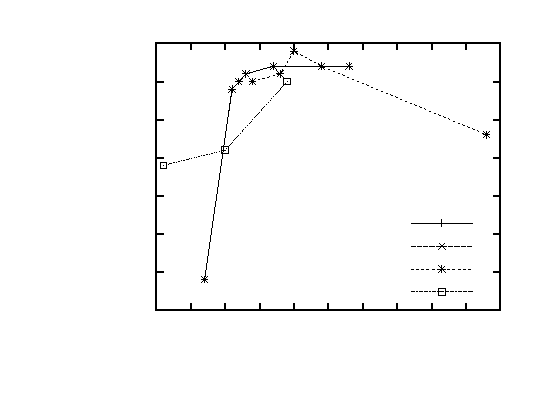
\includegraphics{DCPT-plot}}%
    \gplfronttext
  \end{picture}%
\endgroup

    \caption{Speedup using the DCPT prefetcher}
    \label{graph:dcpt}
\end{center}
\end{figure}
